%!TEX root = ../thesis.tex
\chapter{绪论}

%%%%%%%%%%%%%%%%%%%%%%%%%%%%%%%%%%%%%%%%%%%%%%%%%%%%%%%%%%%%%%%%%%%
\section{选题背景和研究意义}

我国城市轨道交通建设正处于飞速发展的阶段,截止2017年初,中国大陆地区共28个城市启动城市轨道交通运营,总计通车114条线路,运营线路的总长度达到3746公里;在“十二五”期间,累积新投运线路2019km,完成累积投资12289亿元,未来投资将持续增长,如图\ref{fig:城市轨道交通投资额}所示。建设规模居世界之首(轨道城市,\citeyear{轨道2017})。同时,国家发改委、住建部发布了首部国家级市政基础设施规划(住房和城乡建设部,\citeyear{住房和城乡建设部}),中国所倡导的“一带一路”宏伟计划,势必将轨道交通的建设推向一个新的高潮。随着轨道交通的建成与投入运营,作为城市的交通命脉,在100年的设计寿命期内,修筑于岩土介质的盾构隧道结构健康服役性能对于城市正常运转至关重要,越来越受到社会的广泛关注。例如北京、上海、广州等超大城市,一旦城市轨道交通的任一节点出现问题,将波及整个地铁网络,阻碍几百万人的出行,进而造成城市交通系统的瘫痪和恶劣的社会影响。

\begin{figure}[!h]
	\centering
	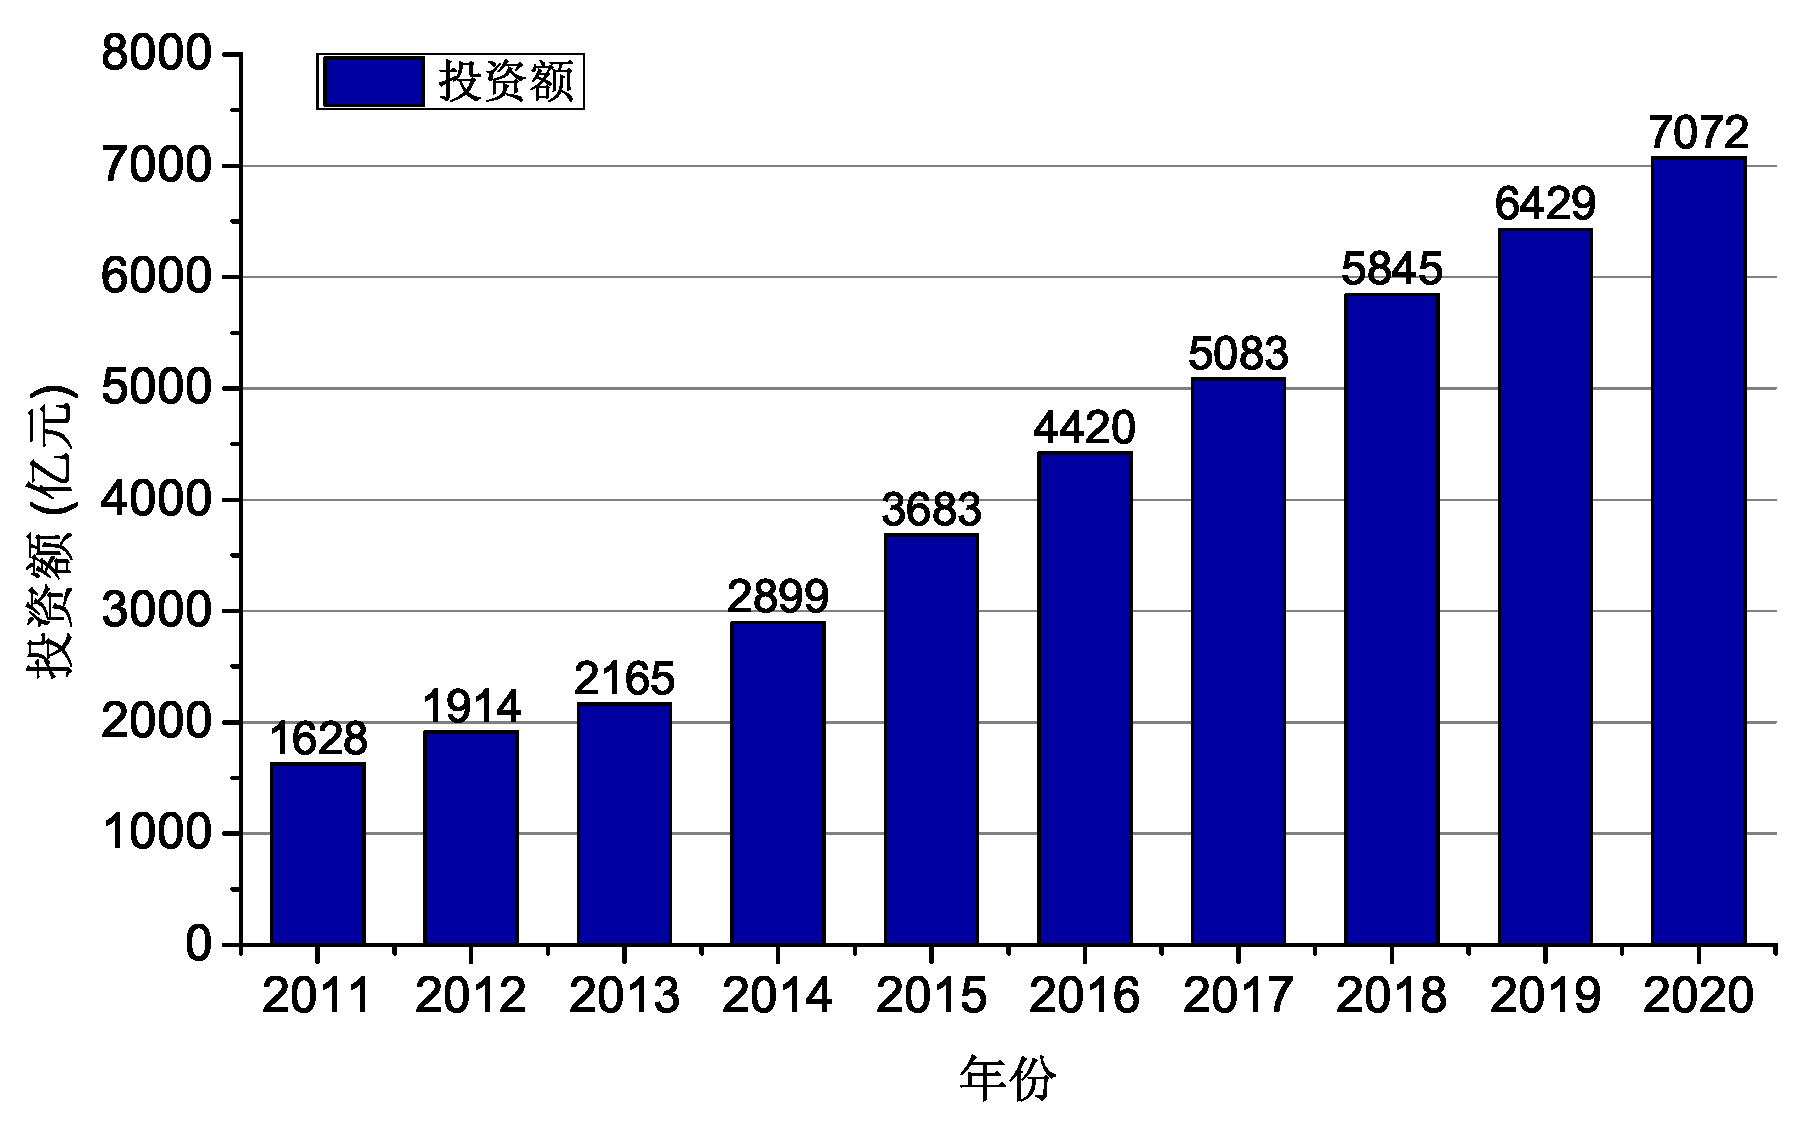
\includegraphics[width=0.7\textwidth]{chap1/investment.eps}
	\caption{中国城市轨道交通投资额}
	\label{fig:城市轨道交通投资额}
\end{figure}

我国城市轨道交通建设发展快但历史短,人们对结构健康服役问题的严重性重视程度不够。作为重大地下工程的城市轨道交通盾构隧道,所处岩土条件复杂、周边环境敏感、列车运行密度极高、使用条件苛刻,结构自身在多因素长期作用下性能不断劣化,一旦损坏不易或不可更换,并将会诱发地下工程灾害,因而对城市轨道交通盾构隧道健康服役提出了极高的要求。目前运营中的城市轨道交通健康服役问题已开始显露。

上世纪70年代建成的香港地铁部分隧道,在90年代就发现内排钢筋严重锈蚀,导致混凝土保护层的剥落,影响到正常使用。2001年5月22日,台北地铁淡水线士林站附近道床发生裂缝,地铁被迫减速,并改为手动驾驶,10万旅客上班受阻。北京地铁第一期工程1971年投入运营数年后,发现严重的杂散电流,已造成主体结构钢筋腐蚀,隧道内水管腐蚀穿孔。2006年8月19日,上海轨道交通2号线河南路-陆家嘴站越江隧道泵站由于振动与结构渗漏水的耦合叠加作用发生涌水冒浆险情,造成停运数小时。2009年12月22日,上海轨道交通1号线由于隧道结构顶部碳纤维脱落造成陕西南路至人民广场区间突发供电触网跳闸故障,造成该区列车停驶,16万人受困于地铁内、数百万人出行受阻,为建国以来城市轨道交通发生的最大事故。 

国外同样,2017年美国土木工程师协会(ASCE,\citeyear{ASCE2017})评价美国土木基础设施的平均等级为D+,估计需要花费20000亿美元才能够挽救这种长期忽视的问题。1999年10月9日,日本山阳城际新干线Kitakyushu隧道发生混凝土掉落击中电网事故,造成多趟列车取消,62000人因此出行受阻,事故调查显示原因是由于混凝土施工过程中存在缺陷,在渗漏、温度变化、列车振动等长期作用下导致裂隙不断发展所致。列宁格勒地铁1号线“森林”车站到“英勇广场”车站区间 1975 年投入运营。1994年隧道(通过钢板隔水层上的卸压排水管)经常间歇性涌水涌砂,1995年12月3日夜,下线隧道大量涌水,上线隧道急剧下沉,1995年12月4日,隧道运营终止。

上述事故表明,城市轨道交通地下结构在服役环境不断变化、材料劣化等内外因素共同作用下,其受力状态会发生变化,性能逐步退化,加之我国轨道交通建设速度迅猛,其结构施工质量难免存在一定程度的缺陷,因而城市轨道交通盾构隧道健康服役面临的问题日益突出。

综上所述,本文的研究意义体现在以下三个方面:(1)盾构隧道服役性能评估与分析有助于延长隧道的使用寿命。在隧道投入运营后,病害的出现势必缩短隧道使用寿命,适时合理的维修有助于延长隧道寿命。通过隧道结构服役性能理论研究,可以指导隧道维修时机,掌握隧道服役性能状况,制定科学的维修加固措施,延长隧道的结构劣化。

(2)盾构隧道服役性能评估与分析有助于提升城市轨道交通的社会形象。隧道作为轨道交通线路的重要一环,其健康安全是整条线路通畅运行的基础,一旦出现安全事故或列车停运,其社会负面影响将是难以估量的,严重时会影响到社会的稳定。因此全面掌握隧道服役性能状态,将安全隐患消灭在萌芽状态,保证线路的安全畅通,具有重大的政治意义。

(3)盾构隧道服役性能评估与分析有助于降低城市轨道交通养护维护成本。目前各国的土建结构维护费改建费增加迅速,维护费用成为财政的巨大负担。由于目前盾构隧道结构健康评估理论的不成熟,导出盲目维修、过度维修的现象,不但使得隧道病害未能得到有效治理,也造成巨大的经济浪费。因此对隧道服役性能的研究,可以以最少的资金投入达到最优的治理效果,具有重大的经济效益。

%%%%%%%%%%%%%%%%%%%%%%%%%%%%%%%%%%%%%%%%%%%%%%%%%%%%%%%%%%%%%%%%%%%
\section{国内外研究现状}
%+++++++++++++++++++++++++++++++++++++++++++++++++++++++++++++++++%
\subsection{盾构隧道服役性能评估进展}

目前隧道的服役性能评估方法大致可以分为三种:(1)基于隧道不同单项指标的劣化程度对隧道结构进行评估,在实际工作中最为常用,各国的隧道养护维护规范、手册均给出不同指标的评判标准;(2)基于历史数据建立数学模型对隧道结构进行综合性评估,如专家打分、决策树、概率论、层次分析法、模糊综合等;(3)基于数值模拟分析的评估方法,通过建立精细化数值模型,分析评估指标的评判标准。

\subsubsection{基于单项指标的评估方法}

日本《公路隧道维持管理便览》(日本公路协会,\citeyear{日本公路协会2000公路隧道维持管理便览})主要从隧道病害的发展和掉落的危险性和紧急程度来划分,根据隧道病害的严重性,从外力、材料劣化以及漏水等三个方面考虑,将评估指标划分为3A、2A、A、B四个等级,给出了衬砌变形、沉降、裂缝、剥落、漏水、湧砂、混凝土强度降低、钢筋锈蚀等指标的评判标准。

美国《公路和铁路交通隧道检查手册》(FHWA,\citeyear{FHWA2005Highway})给出隧道病害检测的一般流程,将隧道病害分为轻度、中度和严重三个等级,并规定了病害定量或者定性的评估标准。同时该手册建立了隧道结构的状态的状态分级标准,总共分为0到9十个级别,但手册只是定性地给出这十个等级的评定标准,并未给出具体的、定量的评价方法。

我国《地铁设计规范》(GB50157,\citeyear{GB501572013})对各类隧道病害指标作了规定,如建议衬砌环的直径变形控制在4-6\%衬砌直径以内;地下车站、连接通道和机电设备集中区段的防水等级应为一级,不允许渗水,结构表面无湿渍,区间隧道及连接通道等附属隧道机构防水等级应为二级,顶部不允许滴漏,其他不允许漏水,结构表面可有少量湿渍;衬砌管片的接缝张开量控制在1-2mm以内等。该规范并未对隧道状态评估进行规定。

我国《盾构法隧道结构服役性能鉴定规范》(DG/TJ08-2123-2013,\citeyear{DGTJ0821232013})根据设计规定、使用时间、使用条件和使用状况,进行结构服役性能鉴定。将隧道结构服役性能等级分级为正常、退化、劣化、恶化、危险五个等级,如表\ref{tab:服役状态等级分级标准}所示。将隧道结构服役状态鉴定分为五个层次,分别为隧道结构使用环境、构件服役状态等级评定、结构连接服役状态等级评定、结构区段服役状态等级评定和隧道整体服役状态等级评定,每一个层次的评定根据上一个层次评定结果所占比例决定。

\begin{table}[htbp]
  \centering
  \caption{盾构隧道服役状态等级分级标准}
    \begin{tabular}{?c"c"m{19.065em}"c?}
    \thickhline
    分级    & 服役状态  & \multicolumn{1}{c"}{分级定义} & 图示色彩 \bigstrut\\
    \thinhline
    i     & 正常    & 结构区段中的构件无安全隐患、无显著变形、无渗漏 & 绿色 \bigstrut\\
    \thinhline
    ii    & 退化    & 结构区段中部分构件耐久性退化,个别构件变形较大或结构连接处渗漏,但构件无安全隐患。 & 蓝色 \bigstrut\\
    \thinhline
    iii   & 劣化    & 结构区段中多数构件的耐久性劣化,整体变形较大或部分结构连接渗漏,但构件无安全隐患。 & 黄色 \bigstrut\\
    \thinhline
    iv    & 恶化    & 结构区段中整体变形较大 或多处结构连接明显渗漏,但无安全隐患。 & 橙色 \bigstrut\\
    \thinhline
    v     & 危险    & 结构区段中构件安全性不足、或结构区段变形过大或结构连接出现线流、漏泥沙。 & 红色 \bigstrut\\
    \thickhline
    \end{tabular}%
  \label{tab:服役状态等级分级标准}%
\end{table}%

\subsubsection{基于数学模型的评估方法}

吴江滨(\citeyear{吴江滨2004铁路运营隧道衬砌状态评估体系的建立及工程应用研究})在收集100余座铁路运营隧道数据基础上,提出隧道衬砌状态的评价体系,各个评价指标的评估标准根据应力集中系数给出,采用层次分析模型对隧道进行评估。但由于评价指标仅仅考虑了衬砌厚度和衬砌背后接触情况,评价指标过少,该评价体系未能很好反映隧道真实状态。

罗鑫(\citeyear{罗鑫2008公路隧道健康状态评估方法及系统研究})根据综合评估指标遴选原则和层次分析法原理,确定并建立了公路隧道结构健康状况综合评估体系,给出了不同评估指标的定量评定标准。采用乘积标度发确定指标的标度权重,再根据指标权重和样本数据,采用人工神经网络和模糊理论确定准则层指标权重,给出了隧道健康状态的模糊综合评价模型。

刘涛(\citeyear{刘涛2008既有盾构隧道结构性能评价研究})研究了现有城市盾构隧道的评估体系构成,和相应的评估工作流程,认为盾构隧道结构服役性能应该包含结构的安全性和耐久性,将评估指标分为整体的性能评估指标、安全性能的评估指标和耐久性的评估指标。并提出盾构隧道衬砌耐久性退化模型,基于Bayesian条件概率对耐久性模型进行修正,采用可靠度理论和Markov链方法对隧道结构的服役性能进行评价。

唐亮(\citeyear{唐亮2008隧道病害调查分析及衬砌结构的风险分析与控制研究})在分析隧道衬砌的主要破坏形式和影响结构安全性的风险因素基础上,设计了隧道风险的评价和接受准则,并根据故障树理论,建立隧道的衬砌结构故障树风险分析方法,对各种基本病害事件发生的概率,计算结构劣化的概率。在此之上,通过事件发生概率,提出可靠度理论的结构失效概率计算方法,辅以蒙特卡罗和有限元分析对隧道失效概率进行分析。

杨彤瑶等(\citeyear{杨彤瑶2013基于改进主元分析方法的隧道应变实时监测预警系统})针对隧道结构的实时监测异常数据分析,提出改进的主成分分析方法,即将将原始数据流空间的变化趋势映射到对应的特征向量空间内,求解稳态特征向量,以瞬时特征向量和稳态特征向量关系,作为判据来对同步多维数据流进行异常变化诊断。在此基础上开发隧道实时监测预警系统,根据实测结果,该方法可以实时准确地反映隧道监测数据的异常变化。

李明等(\citeyear{李明2015基于功效系数法的隧道结构健康监测系统预警研究})引入功效系数法对隧道健康监测中的传感器监测数据的进行加权综合,实现监测数据的实时预警和评价。结合隧道结构健康监测系统特点,提出利用同一时刻所有传感器监测数据来确定结构预警指标体系,解决功效系数法中指标体系选取困难的问题。

Nývlt等(\citeyear{N2011Probabilistic})借鉴航天航空行业的风险分析概念,提出适合在隧道工程领域的风险分析方法,并结合决策树、可靠度理论、最优化方程等方法,建立满足安全风险级别下的成本最优化计算方法,该方法在实际工程应用中能指导养护维护决策,图\ref{fig:隧道风险评估决策树}为盾构隧道风险评估的决策树图。

\begin{figure}[!h]
	\centering
	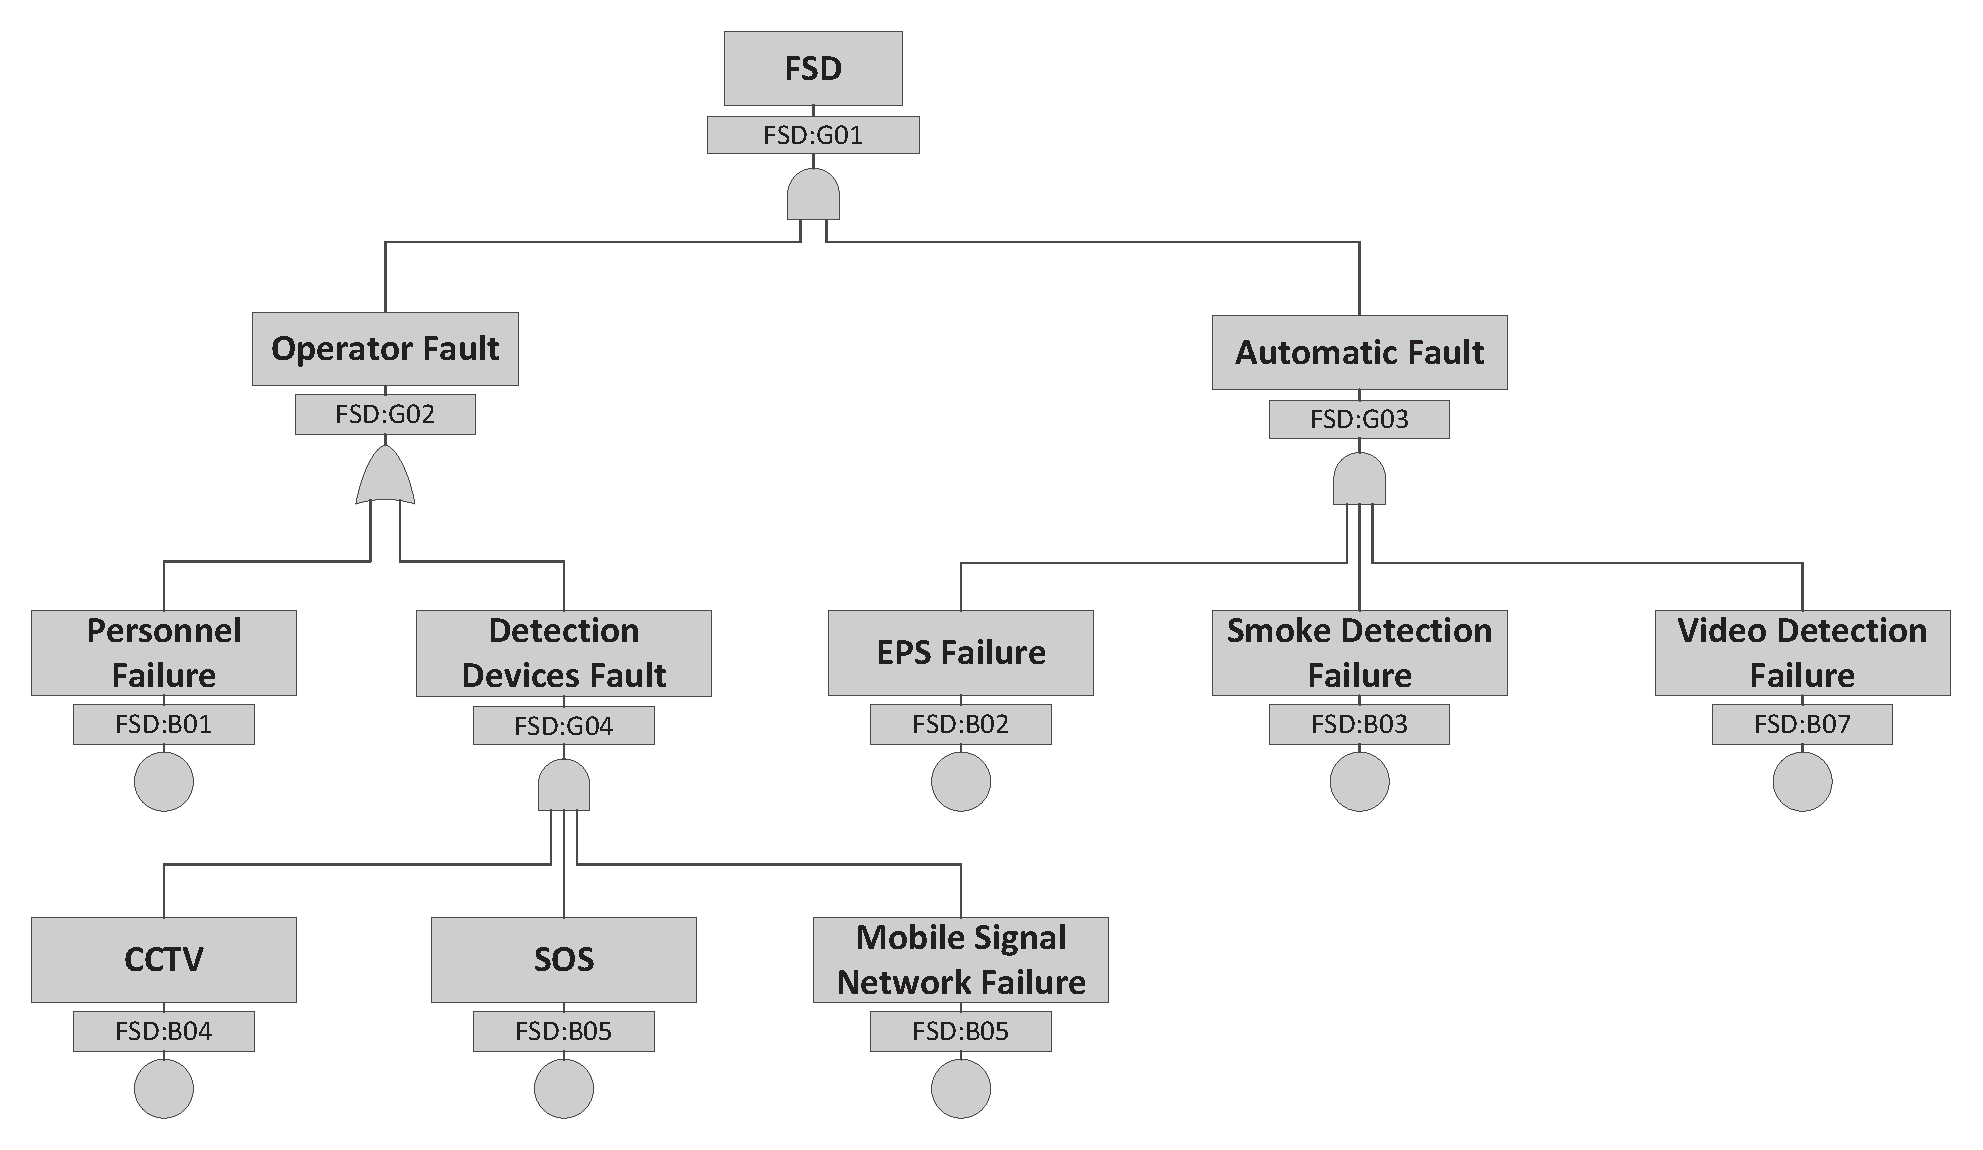
\includegraphics[width=0.9\textwidth]{chap1/nyvlt-faulttree.eps}
	\caption{隧道风险评估决策树}
	\label{fig:隧道风险评估决策树}
\end{figure}

Yuan等(\citeyear{Yuan2012Assessment})为了量化隧道衬砌的结构性能,根据极限状态设计将其分为正常、退化、劣化、恶化、危险五个级别。结构的服役状态包括运营状态和结构状态。其中,运行状态指隧道所处环境条件环境恶劣程度。结构状态指标包括外观性、密封性、完整性、刚性和稳定性。提出了隧道结构服役状态评估的框架,依据运行状态指标和结构指标值与标准值的比较得出其所处的服役状态级别。

Zhang等(\citeyear{Zhang2014Fuzzy})采用模糊分析层次和综合评估模型,合并多个传感器的不同类型的数据,将其映射为盾构隧道的健康评分。选择分段隶属函数,并引入指数量表表征不同权重集。定义模糊运算符号,用于监测因子的模糊综合评估指标。

\subsubsection{基于力学模型的评估方法}

Cavalaro等(\citeyear{Cavalaro2011Structural})研究了施工期盾构隧道衬砌裂缝形成的主要机理,最常见的裂缝是由衬砌之间接触不均匀导致支撑受力不一致而产生的。通过建立不同的有限元模型并对比其分析结果,得出衬砌的接触不均匀直接影响了衬砌的极限承载力。

Naggar和Hinchberger(\citeyear{Naggar2012Approximate})采用数值分析方法,模拟完好的和劣化后的混凝土衬砌力学特性。使用非线性有限元模型模拟混凝土退化,并考虑了土体和混凝土的相互作用和非线性应力应变响应,用于评估劣化后的隧道衬砌的性能状态。

Li等(\citeyear{Li2015Experimental})研究了不同轴向应力水平下弯矩的纵向接缝张开的发展情况和极限状态中的纵向接缝张开,提出了一种渐进模型来预测接缝的力学行为。基于此模型,研究轴向应力水平,螺栓预紧力,混凝土分层深度和螺栓腐蚀深度对接缝力学性能的影响。

Li等(\citeyear{Li2015A})提出了纵缝接头张开的计算模型。模型包含接缝张开不同阶段的不同受力模式,考虑混凝土、螺栓和密封垫对张开量的影响。实验观测与计算分析得出纵缝张开过程可分为四个阶段:阶段一是一开始接缝未张开时,接头处混凝土全截面受压;阶段二接头处混凝土开始出现张开,螺栓拉力逐渐增大;阶段三为外侧边混凝土开始接触;阶段四则是螺栓屈服阶段,如图\ref{fig:接缝张开与弯矩}所示,此模型可用于指导盾构隧道衬砌的接缝张开评估。

\begin{figure}[!h]
	\centering
	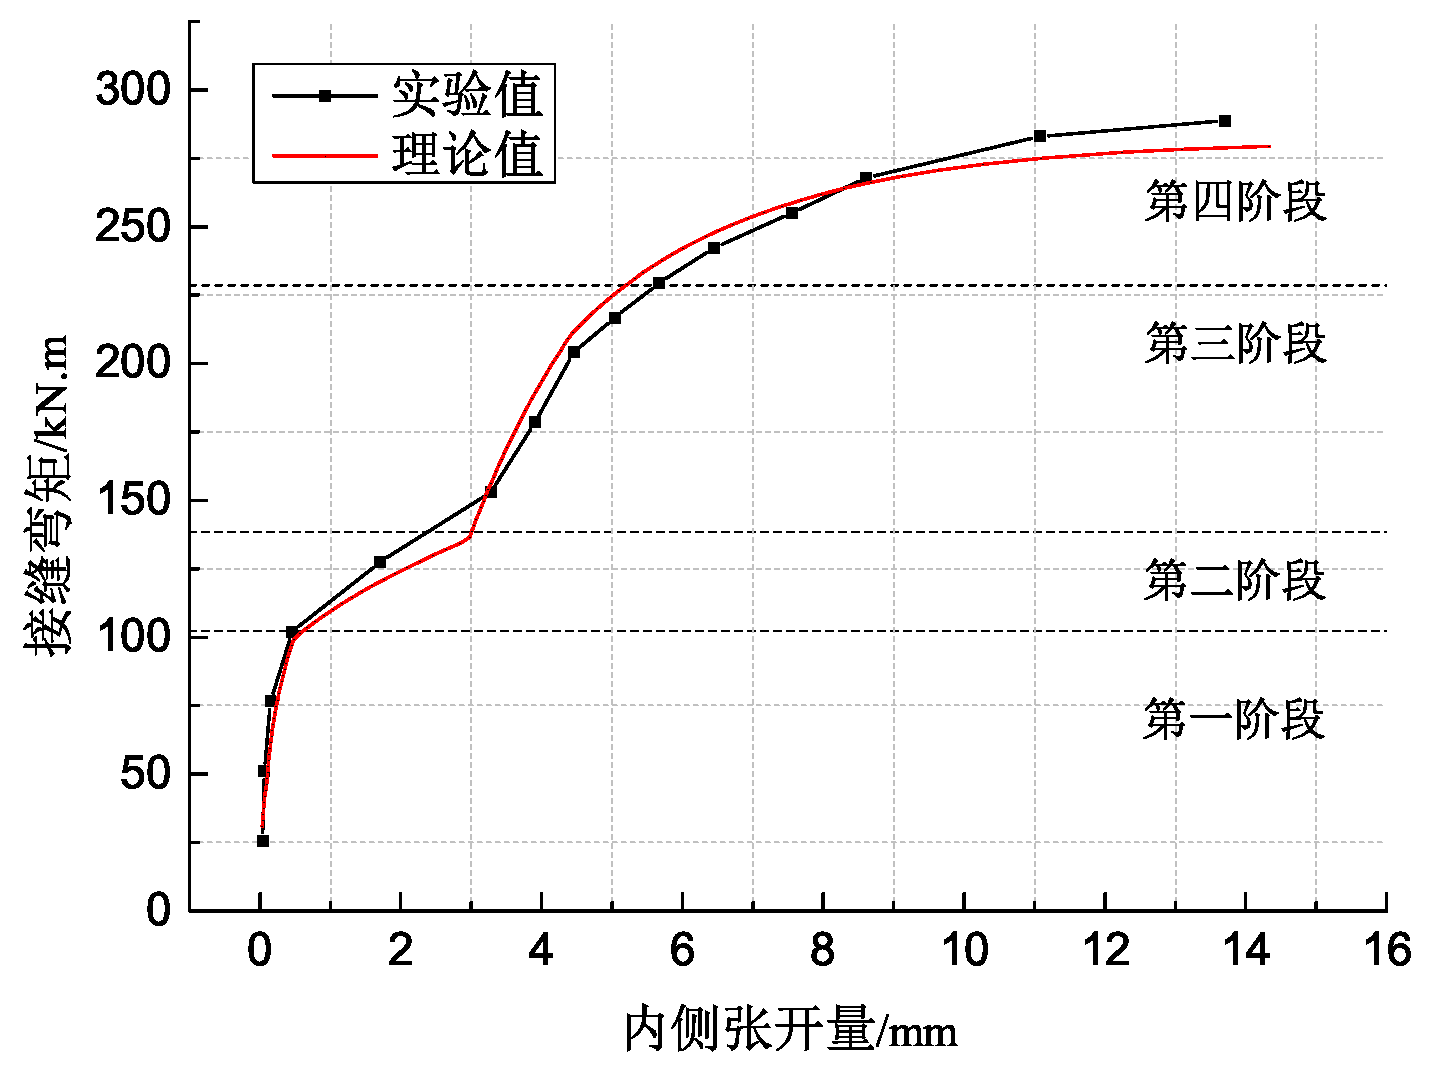
\includegraphics[width=0.7\textwidth]{chap1/joint-moment.eps}
	\caption{盾构隧道衬砌弯矩-接缝张开关系图}
	\label{fig:接缝张开与弯矩}
\end{figure}

袁勇等(\citeyear{袁勇2006运营越江隧道服役现状调查与检测评估})指出对于直径10~m的盾构隧道,隧道的纵向曲率半径小于40~km时,容易导致衬砌环向接头张开增大,引起渗漏。同时渗漏又导致隧道继续产生纵向不均匀变形,二者相互影响。并提出用于既有隧道结构损伤评估的宏观安全性模型和微观耐久性模型。

季倩倩(\citeyear{季倩倩2009带裂缝的盾构隧道衬砌力学模型研究})在盾构隧道的梁-弹簧计算模型中,采用弹簧单元模拟裂缝对衬砌结构的影响,建立了带裂缝的盾构隧道衬砌力学模型。分析结果指出裂缝的存在降低了衬砌的刚度,且降低程度与裂缝宽度和深度相关。

刘曙光(\citeyear{刘曙光2012盾构隧道混凝土管片的承载力退化模型})在现有钢筋混凝土正截面承载力计算方法基础上,考虑了锈蚀钢筋混凝土受弯构件的正截面承载力计算方法,提出盾构隧道衬砌的承载能力退化模型,模型有水平段的诱导期和下降段的劣化期组成,可用于盾构隧道混凝土管片的寿命评估。

王如路和张冬梅(\citeyear{王如路2013超载作用下软土盾构隧道横向变形机理及控制指标研究})采用数值模拟方法分析地面压载、土体侧向压力、土体抗力对盾构隧道收敛变形的影响,给出了收敛变形随压载的变化规律,得出收敛变形与衬砌受力、螺栓受力和接缝张开量的关系曲线,在实际工程中可根据隧道的直径测量量判断隧道的变形状态,为隧道的安全性评价提供指导。

%+++++++++++++++++++++++++++++++++++++++++++++++++++++++++++++++++%
\subsection{盾构隧道服役性能预测进展}

针对盾构隧道结构出现的病害,现有的计算方法还很难全面模拟材料的真实特性、结构与环境的真实状态,因而难以准确评价结构服役性能和确定病害成因、发展趋势及其对服役性能的影响。目前主要有两类方法对盾构隧道服役性能进行预测:(1)考虑材料性能退化的影响,结合盾构隧道数值模型,分析服役性能的退化;(2)基于历史数据,建立数学模型,采用大量数据对模型参数进行估计训练。

\subsubsection{基于材料劣化的性能预测}

Marchand等(\citeyear{Marchand2002Theoretical})研究了弱硫酸根离子对混凝土耐久性的影响,分别试验了水灰比为0.45、0.65、0.75,CSA10和50类型水泥,硫酸盐浓度0-30~mmol/l的不同方案,得出混凝土在硫酸根离子溶液中的退化规律。

Liu等(\citeyear{Liu2014A})考虑早龄期混凝土各组分材料随机分布的影响,及由于水化反应造成的热力学性能时变性和体积变形,将宏观尺度划分为混凝土、砂浆、水泥浆三个不同尺度,对混凝土早龄期性能进行跨尺度研究。建立非线性粘弹性早龄期混凝土多尺度本构模型,并与时间耦合的本构关系。

李忠等(\citeyear{李忠2009氯离子侵蚀盾构隧道衬砌结构性能退化试验})对盾构隧道衬砌钢筋进行加速锈蚀实验,得到不同锈蚀程度的钢筋构件,再对锈蚀钢筋的承载力、变形和破坏特征等作相关测试,获取隧道衬砌结构在氯离子侵蚀下的性能退化规律。

张红光等(\citeyear{张红光2014开裂混凝土内氯离子扩散机理及数值模拟研究})研究得出混凝土结构在初始损伤和裂缝存在情况下,容易造成氯离子等侵蚀性介质在混凝土中快速扩散,通过实验观察和数值模拟,归纳氯离子在混凝土中的扩散系数表达式,为评价混凝土结构的耐久性提供依据。

\subsubsection{基于数学模型的性能预测}

在工程领域,退化模型包括马尔科夫链模型(Madanat等,\citeyear{Madanat1997Probabilistic})、时间序列模型(Prozzi,\citeyear{prozzi2001modeling})、泊松回归模型(Ching和Leu,\citeyear{ching2009bayesian})、灰色预测模型(Wang和Li,\citeyear{wang2011pavement})等,其中马尔科夫链和时间序列最为常用。

Carnahan等(\citeyear{camahan1987optimal})提出马尔科夫链是一种时间离散基于状态的退化模型,其基本假定包括:1)有限个状态;2)状态转移概率只依赖当前的状态;3)转移概率矩阵与时间无关。马尔科夫链模型的转移概率可通过期望值法来估计,但期望值法无法显式地表示影响因素对于状态的影响、考虑退化过程与时间的依赖性、表示连续的退化过程。

Madanat等(\citeyear{Madanat1997Probabilistic}))分别采用了泊松回归模型、有序概率模型来估计马尔科夫链模型中的转移概率矩阵,解决了期望值法无法显式地表示影响因素对于状态的影响、考虑退化过程与时间的依赖性、表示连续的退化过程的问题,可以考虑导致状态变化的影响因素和时间因素。

DeStefano和Grivas(\citeyear{destefano1998method})提出了基于时间的模型以计算状态转移概率。Mishalani和Madanat(\citeyear{mishalani2002computation})提出了基于时间状态离散的随机持续时间模型,能够考虑时间、状态之间的依赖性,表征退化过程与影响因素之间的关系,并且用钢筋混凝土桥面板实例阐述了该方法的可行性。

Chu等(\citeyear{chu2005estimation})提出结构化时间序列模型,该模型可以解释采用不同数据采集方式获取的数据之间的不确定性,同时该模型也可辅助得出维护养护决策时的最优化方案,可以替代传统的马尔科夫链模型。

Chu等(\citeyear{chu2007estimation})采用自回归滑动平均时间序列模型(ARMA 模型)预估基础设施的性能变化,其能考虑状态空间的相互依赖性,预测样本空间外结构的性能变化趋势,也可作为马尔科夫链模型的一种替代方法。

曹净等(\citeyear{曹净2014基于})提出基于小波变换和粒子群优化的最小二乘支持向量机,结合自回归移动平均模型,预测基坑变形的时间序列数据。基于小波变化先将时间序列数据分解为趋势时间序列和随机时间序列两个子序列,分别采用支持向量机和自回归移动平均模型来预测两个子序列,最后再相叠加得到最终预测结果。

文明等(\citeyear{文明2015地铁车站施工过程中地表沉降的})针对时间序列模型的单一线性和忽略外部因素影响的问题,建立了非线性自回归神经网络时间序列模型,如图\ref{fig:非线性自回归神经网络}所示,该模型具有延迟单元和反馈结构,并且可以将外部因素作为外部输入,预测结果适应性更好、准确性更高。

\begin{figure}[!h]
	\centering
	\includegraphics[width=0.9\textwidth]{chap1/NARXNN.pdf}
	\caption{非线性自回归神经网络时间序列模型}
	\label{fig:非线性自回归神经网络}
\end{figure}

%+++++++++++++++++++++++++++++++++++++++++++++++++++++++++++++++++%
\subsection{盾构隧道服役性能服务进展}





%%%%%%%%%%%%%%%%%%%%%%%%%%%%%%%%%%%%%%%%%%%%%%%%%%%%%%%%%%%%%%%%%%%
\section{目前研究存在的问题}




%%%%%%%%%%%%%%%%%%%%%%%%%%%%%%%%%%%%%%%%%%%%%%%%%%%%%%%%%%%%%%%%%%%
\section{论文研究内容、路线和创新点}